\chapter{Introduction to Hamiltonian Systems}
A canonical Hamiltonian system is given by two state variables $p,q \in \mathbb{R}^{n}$ (i.e. the entire system is even dimensional), a \emph{Hamiltonian} function $H(p,q,t)\in \mathcal{C}^{1}(\mathbb{R}^{2n}\times \mathbb{\mathbb{R}})$ which maps $\mathbb{R}^{n}\times\mathbb{R}^{n}\times\mathbb{R}\to \mathbb{R}$. In general $q$ denotes the generalized coordinates (position) and $p$ the generalized momenta. The dynamics on the system is given by
\begin{align}
	\begin{dcases}
		\dot{q} = \frac{\partial H(q,p,t)}{\partial p}\\
		\dot{p} = - \frac{\partial H(q,p,t)}{\partial q}.
	\end{dcases}
\end{align}
This is represented in shorthand notation by using the identity matrix, denoted by $I_{n}\in\mathbb{R}^{n\times n}$ and the symplectic matrix
\begin{align}
	J = 
	\begin{pmatrix}
		0 & I_{n}\\
		-I_{n} & 0
	\end{pmatrix}
.	
\end{align}
Denote the differential with respect to the state variables $x =
\begin{pmatrix}
	p \\ q
\end{pmatrix}
\in \mathbb{R}^{2n}$ by
\begin{align}
	D_{x} = D = 
	\begin{pmatrix}
		\frac{\partial}{\partial q} \\
		\frac{\partial}{\partial p}
	\end{pmatrix}
.	
\end{align}
Then the shorthand notation for the system is
\begin{align}
	\boxed{
	\dot{x} = JD_{x}H(x,t).
}
\end{align}

\begin{ex}[Holonomic mechanical systems are Hamiltonian]
	Assume that all external forces are derived from a potential, i.e. $F(q,t)= -\frac{\partial V(q,t)}{\partial q}$ where $q$ denotes the position. Further assume that all constraints are geometric, i.e. $f(q,t)=0$. We have $n$ degrees of freedom as $q \in \mathbb{R}^{n}$ and $\dot{q} \in \mathbb{R}^{n}$. The kinetic energy is given by $T(q,\dot{q})$ and the potential energy by $V(q,t)$. We then use the principle of least action (also referred to as Hamilton's principle) to derive the equations of motion. This can be shown to be equivalent to Newton's second law. This principle states that for the \emph{Lagrangian} $L(q, \dot{q}, t) = T(q,\dot{q})-V(q,t)$ we have that the variation of the action $S$ is 0
	\begin{align}
		\boxed{
		\delta S = \delta \int_{t_0}^{t_1} L(q(s), \dot{q}(s), s)ds = 0. \numberthis \label{eq8:ELE} 
	}
	\end{align}
	This implies the \emph{Euler-Lagrange equations}
	\begin{align}
\frac{d}{dt} \frac{\partial L}{\partial \dot{q}} - \frac{\partial L}{\partial q} = 0.	
	\end{align}
Thus we have $n$, second-order ODEs. 

\begin{remark}[]
	In \eqref{eq8:ELE} the variation $\delta S$ being equal to 0 stems from the principle of least action, as the action $\int_{}^{} L(q(s), \dot{q}(s), s)ds$ is then a minimum. The variational of a function $\delta F$ (here $F[\gamma]=\int_{}^{} \gamma ds)$ of a path (in our case $\gamma = (q(s), \dot{q}(s), s)$) corresponds to seeing how infinitesimal changes to the path change the output of the functional. These different, admissible paths are depicted in Fig. \ref{fig:variational_deriv}. Hamilton's principle states that among these different paths the one that will physically take place is the one along which the action $S$ is minimal.
	\begin{figure}[h!]
		\centering
		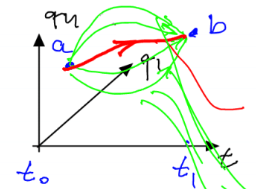
\includegraphics[width=0.35\textwidth]{figures/ch8/1variational_deriv.png}
		\caption{An illustration of various different paths (denoted here by $q(t)$). The red demarcates the actual motion which occurs in the system, whereas the green paths are each admissible motions which are consistent with the constraints.}
		\label{fig:variational_deriv}
	\end{figure}
\end{remark}
Now assume that $L$ is a convex function of $\dot{q}$. Using this the \emph{Legendre transfomation} of $L$ can be performed, which is essentially just a different way to look at the graph of $L(q, \cdot, t)$. This transformation gives us
\begin{align}
	\boxed{H\left(q, \frac{\partial L}{\partial \dot{q}}, t\right) = \frac{\partial L}{\partial \dot{q}}\dot{q} - L(q, \dot{q}, t).} \label{eq8:hamiltonian_def}
\end{align}
Th geometric interpretation of this is shown in Fig. \ref{fig:legendre_trafo}. At each velocity $\dot{q}$ the tangent line of $L(q, \cdot, t)$ is taken and shifted such that the $y$-intercept is at $0$. Then $H$ is equal to the difference between this shifted line and the function $L(q, \dot{q}, t)$.
\begin{figure}[h!]
	\centering
	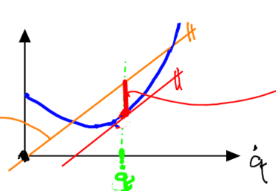
\includegraphics[width=0.35\textwidth]{figures/ch8/2legendre_trafo.png}
	\caption{The Legendre transformation. The thin red linear function denotes the tangent of $L(q, \cdot, t)$ taken at  $\dot{q}$, the yellow linear function is then the shifted version with a 0 $y$-intercept, and the thick red vertical line is the Legendre transformation $H$ measuring the difference between this shifted line and $L(q,\cdot, t)$.}
	\label{fig:legendre_trafo}
\end{figure}

As $L$ is convex, if we define the generalized momenta $p=\frac{\partial L}{\partial \dot{q}}$. There then exists a unique $\dot{q}$ such that $\dot{q} = F(q,p,t)$, in fact the relationship between $\dot{q}$ and $p$ here is bijective. We then have
\begin{align}
	H(q,p,t) = p F(q,p,t) - L (q, F(q,p,t), t)
\end{align}
the Hamiltonian associated with $L$ (or the Legendre transform of $L$).

At this point note that the total differential of $H(q,p,t)$ is
\begin{subequations}
\begin{align}
	dH &= \frac{\partial H}{\partial q}dq + \frac{\partial H}{\partial p}dp + \frac{\partial H}{\partial t}dt \\
	   &= d(pF) - \underbrace{\frac{\partial L}{\partial q}}_{=\dot{p}} dq - \underbrace{\frac{\partial L}{\partial \dot{q}}}_{=p} - \frac{\partial L}{\partial t}dt \\
	   &= \underbrace{F}_{=\dot{q}}dp + pdF - \dot{p}dq - pdF - \frac{\partial L}{\partial t}dt \\
	   &= \dot{q}dp - \dot{p}dq - \frac{\partial L}{\partial t}dt.
\end{align}
\end{subequations}
Comparing coefficients in the first and last equations then yields
\begin{align}
	\begin{dcases}
		\dot{q} = \frac{\partial H}{\partial p}\\
		\dot{p} = -\frac{\partial H}{\partial q}
	\end{dcases}
.	
\end{align}
This first-order ODE is called the \emph{Hamiltonian equations of motion}. The physical meaning of the Hamiltonian can be seen by substituting $L = T(q,\dot{q}) - V(q, t)$ into the definition \ref{eq8:hamiltonian_def}. The kinetic energy only depends on $\dot q$ through the kinetic energy, 
\begin{align}
\dot{q}\frac{\partial L}{\partial \dot{q}} = \dot{q} \frac{\partial T}{\partial \dot{q}}.
\end{align}
Since the kinetic energy is quadratic in the velocity, this simplifies to 
\begin{align}
\dot{q} \frac{\partial T}{\partial \dot{q}} = 2T(q,\dot{q}).
\end{align}
We then have 
\begin{align}
H = 2T - (T - V) = T(q, p) + V(q,t),
\end{align}
which is the full mechanical energy. Also note that we have $\frac{\partial H}{\partial t} = - \frac{\partial L}{\partial t}$.
\end{ex}

We will now apply this result to a well known system.

\begin{ex}[The Hamiltonian of the pendulum]
	Recall that for the pendulum the position is given by $q=\varphi\in S^{1}$, with a string of length $\ell$ the vertical deflection of the pendulum is $\ell(1- \cos(\varphi)$. The string is assumed massless and the mass at the end of the string is given by $m$. 
	
	We have the kinetic and potential energies
	\begin{align}
		T = T(\dot{q}) = \frac{1}{2} m (\ell \dot{\varphi})^{2} = \frac{1}{2} m\ell^2 \dot{\varphi}^{2};\quad V = V(q) = mg\ell(1-\cos(\varphi)).
	\end{align}
Therefore the Lagrangian is given by
\begin{align}
	L = T-V = \frac{1}{2}m \ell^2 \dot{\varphi}^{2} - mg\ell(1-\cos(\varphi)).
\end{align}
To find the generalized momentum, we calculate the partial derivative of the Lagrangian with respect to $\dot{q}$, i.e.
\begin{align}
p = \frac{\partial L}{\partial \dot{q}} = \frac{\partial L}{\partial \dot{\varphi}} = m\ell^2 \dot{\varphi}\implies \dot{\varphi} = \frac{p}{m\ell^2}.
\end{align}
Now it is possible to calculate the Hamiltonian
\begin{align}
	H = p \frac{p}{m\ell^2} - \frac{1}{2}m\ell^2 \frac{p^2}{(m\ell^2)^2} + mg\ell(1-\cos(\varphi))
	= \underbrace{\frac{1}{2} \frac{p^2}{m\ell^2}}_{T} + \underbrace{mg\ell(1-\cos(\varphi))}_{V}.
\end{align}
Hence for this Hamiltonian system we have the Hamiltonian equations of motion
\begin{align}
\begin{dcases}
	\dot{\varphi} = \frac{\partial H}{\partial p} = \frac{p}{m\ell^2} \\
	\dot{p} = - \frac{\partial H}{\partial q} = -mg\ell \sin (\varphi).
\end{dcases}
\end{align}
\end{ex}

\begin{ex}[2-dimensional incompressible fluids are Hamiltonian]
	We begin on a domain $\mathcal{D}$ contained on the plane which is simply connected, i.e. it has no holes. For each position $x\in \mathcal{D}$ we have the velocity field
	\begin{align}
		{V}(x,t) = 
		\begin{pmatrix}
			u(x,y,t) \\ v(x,y,t)
		\end{pmatrix},
	\end{align}
	i.e. for each position we have
	 \begin{align}
		\begin{pmatrix}
			\dot{x} \\ \dot{y}
		\end{pmatrix}
		= 
		\begin{pmatrix}
			u \\v
		\end{pmatrix}
		.
	\end{align}
The incompressibility condition is given by 
\begin{align}
	\nabla \cdot V = \frac{\partial u}{\partial x} + \frac{\partial v}{\partial y}= 0\quad \forall x\in \mathcal{D}\subset \mathbb{R}^{2}. \label{eq8:incompressibility}
\end{align}
Now rewrite \eqref{eq8:incompressibility} in terms of a three dimensional vector field as
\begin{align}
	\nabla \times 
	\begin{pmatrix}
		-v \\ u \\ 0 
	\end{pmatrix}
	=0 \Leftrightarrow
	\nabla \cdot V = 0.
\end{align}
The third component is calculated as $\frac{\partial u}{\partial x} - \frac{\partial (-v)}{\partial y} = \frac{\partial u}{\partial x} + \frac{\partial v}{\partial y} = 0$. On $\mathcal{D}\times \mathbb{R}$ (which is simply connected in $\mathbb{R}^{3}$) the vector field $
\begin{pmatrix}
	-v \\ u \\ 0
\end{pmatrix}
$ has zero curl. Therefore there exists a potential of this vector field $\Psi:\mathcal{D}\times \mathbb{R} \to \mathbb{R}$ such that
\begin{align}
\begin{pmatrix}
	-v \\ u \\ 0 
\end{pmatrix}
 = \nabla \Psi =
 \begin{pmatrix}
 	\partial_x \Psi \\ \partial_y \Psi \\ \partial_z \Psi
 \end{pmatrix}.
\end{align}
Because of the third equation $\Psi$ has no z dependence and we can write our potential as $\Psi = \Psi(x, y, t)$. Therefore we find
\begin{align}
	\begin{dcases}
		-\dot{y} = \frac{\partial \Psi}{\partial x} \\
		\dot{x} = \frac{\partial \Psi}{\partial y}
	\end{dcases}
	\implies 
	\begin{dcases}
		\dot{x} = \frac{\partial \Psi(x,y,t)}{\partial y} \\
	\dot{y} = -\frac{\partial \Psi(x,y,t)}{\partial x}.
	\end{dcases}
\end{align}
Thus we have shown that particle motion is Hamiltonian.
\end{ex}

\begin{ex}[Planar, autonomous dynamical systems with a conserved quantity are Hamiltonian]
	We begin with the dynamical system which has a first integral $U$ (which is not constant), i.e.
	\begin{align}
		\dot{x} = f(x);\quad x \in \mathbb{R}^{2};\quad \exists U:\mathbb{R}^{2}\to \mathbb{R}:\ \frac{dU(x(t))}{dt}=0.
	\end{align}
	Note that this first integral property has further implications
	\begin{align}
		\frac{dU(x(t))}{dt} = DU(x(t)) \cdot \dot{x}(t) = DU \cdot \left.f\right|_{x(t)} = 0 \implies DU \perp f.
	\end{align}
Therefore, we can take the orthogonal complement of $DU$ and scale this to be equal to $f$, i.e.
\begin{align}
	f(x) = p(x) JDU(x) \implies \dot{x} = p(x) JDU(x).
\end{align}
Such a system is called a \emph{generalized Hamiltonian system} with the scalar function $p(x)$. Here the symplectic matrix in 2 dimensions is given by the $90^{\degree}$ rotation
\begin{align}
	J = 
	\begin{pmatrix}
		0 & I_{1}\\
		-I_{1} & 0 
	\end{pmatrix}
	=
	\begin{pmatrix}
		0 & 1 \\
		-1 & 0
	\end{pmatrix}
	.
\end{align}
If we assume $p(x)\neq0$ for all $x\in \mathcal{D} \subset \mathbb{R}^{2}$ then we may define the trajectory-dependent rescaling of time
\begin{align}
	\tau = \int_{0}^{t} p(x(s))ds.
\end{align}
Then, define the notation for the derivative with respect to $\tau$ as follows
 \begin{align}
	 \frac{d(\ )}{dt} = \frac{d(\ )}{d\tau} \underbrace{\frac{d\tau }{dt}}_{p(x(t))} = (\ )' p.
\end{align}
Hence, using this time-transformation we have
\begin{align}
	\dot{x} = pJDU \implies x'p = pJDU \implies \boxed{x' = JDU(x).}
\end{align}
Therefore, we have a canonical Hamiltonian system. In fact, all planar, autonomous systems with a nontrivial first integral are Hamiltonian systems after a possible reparameterization of time.
\end{ex}

\begin{remark}[]
	The fact that the first integral was not trivial (i.e. non-constant) is critical, as otherwise $DU$ would be constantly 0, as we must be able to phrase the right hand side $f$ in terms of $DU$. Only in the case $f=0$ would this then be possible.
\end{remark}

\begin{ex}[Lotka-Volterra model (1925) for predator-prey interactions]
	For more information about this model see \cite{Lotka1925, Volterra1926}. Let the size of the prey population be represented by $h(t)$ and the size of the predator population be denoted by $p(t)$. Each of these populations must be at least 0. Now for strictly positive constants $a_1$, $a_2$, $b$, and $c$ we have the following dynamics
	\begin{align}
		\begin{dcases}
			\dot{h} = a_1 h(1- bp) \\
			\dot{p} = -a_2 p(1-ch).
		\end{dcases}
	\end{align}
	The phase portrait of this system is depicted in Fig. \ref{fig:lotka_volterra}.
	\begin{figure}[h!]
		\centering
		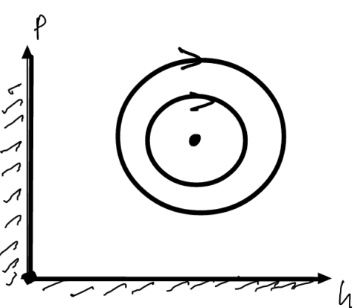
\includegraphics[width=0.3\textwidth]{figures/ch8/3lotka_volterra.png}
		\caption{The phase portrait of the Lotka-Volterra dynamics, which has been used to explain the observed cycles in fish populations.}
		\label{fig:lotka_volterra}
	\end{figure}

	This system does in fact have a first integral, and thus it is Hamiltonian.	
\end{ex}

Now that we have seen multiple examples of Hamiltonian systems, we would like to better understand what properties they all share.

\section{Properties of Hamiltonian systems}
The setup going forward will be as follows for $n\geq 1$
\begin{align}
	\dot{x} = JDH(x,t);\quad x=
	\begin{pmatrix}
		q \\ p
	\end{pmatrix}
	\in \mathbb{R}^{2n};\quad 
	J=
	\begin{pmatrix}
		0 & I_n\\
		-I_n & 0 
	\end{pmatrix}.\numberthis \label{eq8:hamiltonian}	
\end{align}
\begin{proposition}[Conservation of the Hamiltonian (energy)]
	If $\frac{\partial H}{\partial t}=0$ (i.e. $H$ is only a function of $q$ and $p$) then $H(x(t))$ is constant on all trajectories. Therefore $H(x)$ is a first integral.	
\end{proposition}
\begin{proof}
	Use $J = -J^{T}$ to calculate
	\begin{align}
		\frac{dH(x(t))}{dt} = DH(x(t)) \cdot JDH(x(t)) = \left.\langle DH, JDH \rangle \right|_{x= x(t)} = 0.
	\end{align}
\end{proof}
The \emph{energy surface} for some constant $E_{0}=\left\{ x \in \mathbb{R}^{2n}:\ H(x)= H_0 \right\} $, for some constant $H_0$, is an invariant surface for the system. By nature of this $JDH$ must be tangent to $E_0$. Assuming that $E_0$ contains no fixed points of \eqref{eq8:hamiltonian} is equivalent to $DH(x_0)\neq 0$ for all $x_0$ in $E_0$. Hence, by the Implicit Function Theorem, the solution of $H(x)-H_0=0$ can be smoothly continued from $x_0$. Indeed, we have
\begin{align}
	DH(x_0)\neq 0\in \mathbb{R}^{2n} \implies \exists i:\ \left.\frac{\partial H}{\partial x^{i}}\right|_{x=x_0} \neq 0.
\end{align}
Then we have $x^{i}=F\left(x^{1},\ldots,x^{i-1},x^{i+1},\ldots,x^{2n}\right)$ for $F\in \mathcal{C}^{1}$, because $H$ is smooth. This implies that $E_{0}$ is a smooth $2n-1$-dimensional graph (i.e. a smooth hypersurface or codimension-one surface).

\begin{ex}[Two degree of freedom nonlinear oscillator]
	Between two fixed sides, three nonlinear springs hold two masses. Each spring has a potential given by $V_{i}$ for $i=1,2,3$ and the masses are given by $m_1$ and $m_2$. The displacement of each mass is given by $q_1$ and $q_2$ respectively. The potentials have global minima at $x=(q_1, q_2)^T=0$, and are otherwise strictly monotone. The system and example potential are illustrated in Fig. \ref{fig:2dof_oscillator_hamiltonian}.
	\begin{figure}[h!]
		\centering
		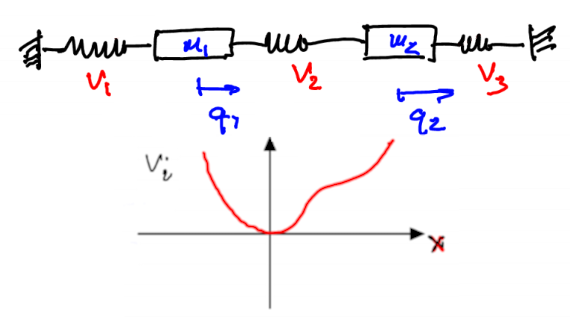
\includegraphics[width=0.5\textwidth]{figures/ch8/4_2dof_oscillator_hamiltonian.png}
		\caption{The two degree of freedom nonlinear oscillator and an example of a potential $V_i$.}
		\label{fig:2dof_oscillator_hamiltonian}
	\end{figure}
	
	For this system the specific conditions on the potentials are
	\begin{align}
		V_{i}(0) =0;\quad V_{i}'(0)=0;\quad V_{i}''(0)>0;\quad \forall x\neq 0:\ V_{i}''(x)\neq 0 . \label{eq8:2dof_conditions}
	\end{align}

	The Lagrangian is then
	\begin{align}
		L=T-V = \frac{1}{2} m_1 \dot{q}_{1}^{2} + \frac{1}{2}m_2 \dot{q}_{2}^{2} - \left[V_1(q_1) + V_2(q_2 - q_1) + V_3(-q_2) \right].
	\end{align}
From the Lagrangian the generalized momenta can be derived
\begin{align}
	p_i = \frac{\partial L}{\partial \dot{q}_{i}} = m_{i} \dot{q}_{i} \implies \dot{q}_{i} = \frac{p_i}{m_i}\quad i=1,2.
\end{align}
And with this the Hamiltonian can be calculated as
\begin{align}
	H = T+V = \frac{1}{2}\frac{p_1^{2}}{m_1} + \frac{1}{2}\frac{p_{2}^{2}}{m_{2}} + V_1(q_1) + V_2(q_2 - q_1) +V_{3}(-q_2).
\end{align}
Now recall that $\dot{x}=JDH(x)$, therefore the fixed point $x_0=(q^{0}, p^{0})^{T}$ can be found by identifying the roots of $DH$ 
\begin{align}
	DH(x_0)=0 \Leftrightarrow
	\begin{pmatrix}
		V_{1}'(q_{1}^{0}) - V_{2}'(q_{2}^{0} - q_{1}^{0}) \\
		V_{2}'(q_{2}^{0} - q_{1}^{0}) - V_{3}'(-q_{2}^{0}) \\
		\frac{p_{1}^0}{m_1} \\
		\frac{p_{2}^{0}}{m_2}
	\end{pmatrix}.
\end{align}
For instance the origin is a fixed point, i.e.
\begin{align}
	x_0 = 
	\begin{pmatrix}
		q^{0} \\ p^{0}
	\end{pmatrix}
	=0\in \mathbb{R}^{4}.
\end{align}
Hence we have
\begin{align}
	p_{1}^{0} = p_{2}^{0}= 0;\quad V_{1}'(q_{1}^{0}) = V_{2}^{1}(q_2^{0}-q_{1}^{0});\quad V_{2}'(q_{2}^{0}-q_{1}^{0})=V_{3}'(-q_{2}^{0}) \label{eq8:2dof_star}.
\end{align}
Assume that $q_{1}^{0}>0$ solves \eqref{eq8:2dof_star}. Then we would have the following
\begin{align}
	V_{1}'(q_{1}^{0}) = V_{2}'(q_{2}^{0} - q_{1}^{0}) > 0 \implies q_{2}^{0}>q_{1}^{0} >0,
\end{align}
due to the conditions set out in \eqref{eq8:2dof_conditions}. However we also have that
\begin{align}
	V_{3}'(-q_{2}^{0}) = V_{2}'(q_{2}^{0}-q_{1}^{0})>0 \implies -q_{2}^{0}>0.
\end{align}
These two inequalities are clearly in contradiction. A similar argument shows that $q_{1}^{0} < 0$ also leads to a contradiction. Therefore we find that at all equilibria $q_{1}^{0}=0$ and by symmetry $q_{2}^{0}=0$ as well. Thus the only fixed point is given by $q_{1}^{0}=q_{2}^{0}=0$ and $p_{1}^{0}=p_{2}^{0}=0$. We can conclude that all nonzero energy surfaces are codimension-one (3-dimensional) invariant manifolds (i.e. smooth surfaces).

Now it is possible to analyze the stability of this fixed point. To use Lyapunov's direct method, the Hamiltonian is a good candidate for a Lyapunov function, because $H(0)=0$, $DH(0) = 0 \in \mathbb{R}^{4}$, and $\frac{dH(x(t))}{dt}=0$. We still need to find out if $H$ is cup shaped. First calculate the Hessian
\begin{align}
	D^2H = 
	\left(
	\begin{array}{c|c}
		D^2V & 0_{2\times 2} \\
		\hline
		0_{2\times 2} &
		\begin{array}{c c}
			\frac{1}{m_1} & 0 \\
			0 & \frac{1}{m_2}
		\end{array}
	\end{array}
\right)
.
\end{align}
Next, we evaluate if each of the diagonal matrices are positive definite. The lower right matrix is clearly positive definite as it is a diagonal matrix with strictly positive entries. For the upper left, a calculation is required
\begin{align}
\left.D^2V\right|_{0} = 
	\left.\begin{pmatrix}
		V_{1}'' + V_{2}'' & -V_{2}'' \\
		-V_{2}'' & V_{2}'' + V_{3}''
	\end{pmatrix} \right|_{x = 0 \in \mathbb{R}^{4}}.
\end{align}
Due to the fact that $\left. V_{1}'' + V_{2}''\right|_{0}>0$ and $\det\left(\left.D^2V\right|_{0}\right) >0$ we have that $\left.D^2V\right|_{0}$ is positive definite by Sylvester's theorem. Hence $D^2H$ is positive definite, i.e. cup shaped. Now we have shown that $H(x)$ is a Lyapunov function, and therefore guarantees that the origin is nonlinearly stable irrespective of the actual form of the potentials. 

From this we wonder what else can be said about the global phase space geometry, which leads us to the Morse lemma.
\begin{lemma}[Morse]
Let $x_0$ be a nondegenerate critical point for $f:\mathbb{R}^{n}\to \mathbb{R}$, i.e 
\begin{align}
	Df(x_0) =0,\quad \det\left(D^{2}f(x_0)\right)\neq 0.
\end{align}
Let $k$ be the number of negative eigenvalues of $D^2f(x_0)$. Then there exists a local change of coordinates (diffeomorphism) $x\mapsto y$ near $x_0 $ such that in the new coordinates
\begin{align}
	f(y) = f(x_0) - y_1^{2} - \ldots - y_{k}^{2} + y_{k+1}^{2} + \ldots +y_{n}^{2}.
\end{align}
\end{lemma}

By the Morse lemma, there exists a change of coordinates $x\mapsto y$ such that $H(y) = y_{1}^{2} + y_{2}^{2} + y_{3}^{2}+y_{4}^{2}$ that is suitable near the origin. Therefore the energy surface $E_{h_0} = \left\{ y \in \mathbb{R}^{4}:\ H(y) = h_0\right\}$ is equal to $\mathcal{S}^3 \subset \mathbb{R}^{4}$, where $\mathcal{S}^{3}$ is the 3-dimensional hyper-sphere. This means in the original $x$-coordinates, all low-energy level sets of $H(x)$ are diffeomorphic to $3$-dimensional spheres.
\end{ex}

It is possible to draw on other results from differential geometry, namely the foliation theorem \cite{Milnor1965}. This tells us that level surfaces of a scalar function can only change their topology (i.e. become no longer diffeomorphic to each other) through level surfaces that contain a critical point of the function ($Df$ must vanish somewhere on the level set). 

We can see this in the example of the pendulum equation, whose Hamiltonian we previously derived. The stable fixed point is a nondegenerate critical point of the Hamiltonian (as all other points around it have more energy) and by the Morse lemma, after a change of coordinates, level surfaces can be parametrized as a sum of quadratic terms. The loops representing periodic oscillation are also the level sets for the respective energy level and are all diffeomorphic to each other (they are all diffeomorphic to $\mathcal{S}^{1}$) until the level set which intersects the unstable fixed points. This transition is depicted in Fig. \ref{fig:morse_foliation}.

\begin{figure}[h!]
	\centering
	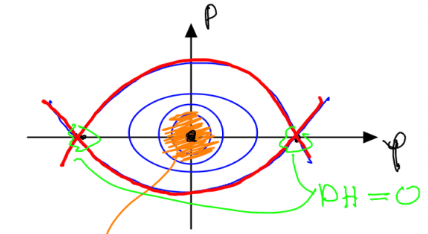
\includegraphics[width=0.4\textwidth]{figures/ch8/5morse_foliation.png}
	\caption{The effect of the foliation theorem. Around the stable fixed point where the Morse lemma applies is shaded orange, and the level sets containing critical points of $H$.}
	\label{fig:morse_foliation}
\end{figure}

Regarding the two degree of freedom oscillator example previously handled, all surfaces are diffeomorphic to $\mathcal{S}^{3}$ as $x=0$ is the only critical point of $H$.

\section{Volumes under Hamiltonian flow maps}
We would like to understand what happens with a volume of the phase space under the flow map of a Hamiltonian system. When we talk about the transformation of a volume $V(t_0)$ under the flow map, we mean to study the set $V(t)$ which results from applying the flow map to $V(t_0)$, i.e. $V(t) = F_{t_0}^{t}(V(t_0))$. The evolution of such a volume in shown in Fig. \ref{fig:vol_change}. However, before continuing to study this, we must prove Liouville's theorem.
\begin{figure}[h!]
	\centering
	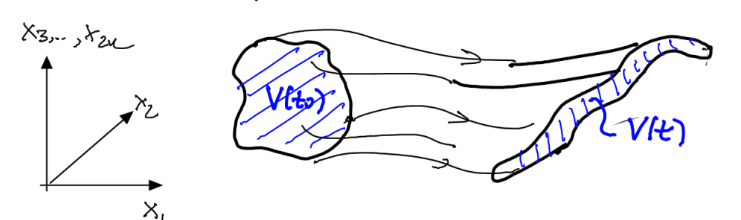
\includegraphics[width=0.6\textwidth]{figures/ch8/6vol_change.png}
	\caption{A transformed volume of the phase space under the flow map.}
	\label{fig:vol_change}
\end{figure}

\begin{theorem}[Liouville]
	For a dynamical system
	\begin{align}
		\dot{x} = f(x,t);\quad x \in \mathbb{R}^{n};\quad f\in\mathcal{C}^{1},
	\end{align}
	we have that
	\begin{align}
		\boxed{
			\frac{d}{dt} \textrm{vol} (V(t)) = \int_{V(t)}^{} \nabla \cdot f(x,t) dV.
		}
	\end{align}
\end{theorem}
\begin{proof}
	Calculate the equation of variations for this system with $x(t) = x(t;t_0, x_0)$
	\begin{align}
		\frac{d}{dt}\frac{\partial {x}}{\partial x_0} = Df(x(t),t) \frac{\partial x}{\partial x_0} \implies \frac{d}{dt}\left[ \frac{\partial x}{\partial x_0}\right] = \underbrace{Df(x(t),t)}_{A(t)}\frac{\partial x}{\partial x_0}.
	\end{align}
	This measures how sensitive the resulting $x(t)$ is on the initial condition $x_0$. We can generalize this to 
	\begin{align}
		\dot{X} = A(t) X;\quad A(t) = Df(x(t),t);\quad X,A \in \mathbb{R}^{n\times n}.
	\end{align}
	The only consistent initial condition for this is $\left.\frac{\partial x}{\partial x_0}\right|_{t=t_0}=X(t_0) = I_{n} \in \mathbb{R}^{n\times n}$. Recalling Abel's theorem, which applies to \underline{any} linear system of ODE's we have
		\begin{align}
			\det(\underbrace{X(t)}_{DF_{t_0}^{t}}) = \det(\underbrace{X(t_0)}_{I_{n}})\cdot \exp\left(\int_{t_0}^{t} \ \textrm{Tr} [A(s)]ds\right).
		\end{align}
	Note that in present case $\frac{\partial x}{\partial x_0}=DF_{t_0}^{t}$. Finally, for a general dynamical system we have
	\begin{align}
		\det\left(DF_{t_0}^{t}\right) = \exp \left( \int_{t_0}^{t} \nabla \cdot f(x(s), s) ds \right).
	\end{align}
	Using this we calculate
\begin{subequations}
	\begin{align}
		\frac{d}{dt}  \textrm{vol}\left[V(t)\right] 
		&= \frac{d}{dt}\int_{V(t)}^{} dV 
		= \frac{d}{dt} \int_{V(t_0)}^{} \det\left(DF_{t_0}^{t}(x_0) \right) dV_0 \\
		&= \int_{V(t_0)}^{} \frac{d}{dt}\det\left(DF_{t_0}^{t}(x_0) \right) dV_0
		= \int_{V(t_0)}^{} \nabla \cdot f(x(t),t) \underbrace{\det\left(DF_{t_0}^{t}\right) dV_0}_{=dV}\\
		&= \int_{V(t)}^{} \nabla \cdot f(x(t),t) dV.
	\end{align}
\end{subequations}
Where on the last equation of the first line we used the change of coordinates $y = F_{t_0}^{t}(x_0)$, then on the last equation of the second line we used our previous result, and then finally switched back to the original coordinates for the final equality.	
\end{proof}


\begin{proposition}[Conservation of phase space volume]
	For any Hamiltonian system, the flow map $F_{t_0}^{t}:x_0 \mapsto x(t;t_0,x_0)$ is volume preserving for any $t_0, t \in \mathbb{R}$. 
\end{proposition}
\begin{proof}
	For Hamiltonian systems we have that
	\begin{subequations}
	\begin{align}
		\nabla \cdot (\underbrace{JDH(x,t)}_{f(x,t)}) &=  \textrm{Tr} \left[ JD^2H(x,t) \right] =  \textrm{Tr} \left[
			\begin{pmatrix}
				0 & I_{n} \\
				-I_{n} & 0 
			\end{pmatrix}
			\begin{pmatrix}
				D^{2}_{qq}H & D^{2}_{qp}H \\
				D^{2}_{qp}H & D^{2}_{pp}H
			\end{pmatrix}
		\right]
	\\
	&= \textrm{Tr} \left[
			\begin{pmatrix}
				D^{2}_{qp}H& *\\
					 * & - D^{2}_{qp}H
		\end{pmatrix} \right]
			=0.
	\end{align}
	\end{subequations}
	Therefore by Liouville's theorem we have that $ \textrm{vol} [V(t)]$ is constant which is equivalent to $\det\left(DF_{t_0}^{t}(x_0)\right)=1$. This is called this \emph{infitesimal (local) form}.
\end{proof}

\section{Consequences of area preservation}
We now constrain ourselves to two dimensional, time-periodic Hamiltonian systems
\begin{align}
	\dot{x}= JDH(x,t);\quad x \in \mathbb{R}^{2};\quad H(x,t)= H(x,t+T);\quad T>0.
\end{align}
The Poincaré map is 
\begin{align}
	P_{t_0}:x_0 \mapsto x(t_0+T; t_0, x_0) = F_{t_0}^{t_0+T}(x_0).
\end{align}
\begin{align}
	H(x,t) = H(x_0) + \varepsilon H_{1}(x,t);\quad x = 
	\begin{pmatrix}
		\varphi \\ p_\varphi
	\end{pmatrix};\quad
	\dot{x} = JDH(x,t),
\end{align}
where $H_1$ and $H$ are $T$-periodic in $t$.

It is possible to classify the different types of fixed points for $P_{t_0}$. Let $x_0$ be a fixed point of $P_{t_0}$, i.e. $P_{t_0}(x_0) = x_0$, then we have by area preservation that
\begin{align}
	\det\left( \left.DP_{t_0}\right|_{x_0}\right) = \det\left( DF_{t_0}^{t_0 + T}(x_0) \right) = 1.
\end{align}
Hence, the eigenvalues $\lambda_1, \lambda_2\in \mathbb{C}$ of the linearized Poincaré map have the property 
\begin{align}
	1 = \det\left(DP_{t_0}(x_0)\right) = \lambda_1 \lambda_2.
\end{align}
Furthermore, as the matrix $D P_{t_0}(x_0)$ is real and has even dimensions, the eigenvalues must occur in complex conjugate pairs.
This implies that there are only a few restricted eigenvalue configurations which are possible.
\begin{enumerate}
	\item \textbf{Robust (structurally stable) configurations} Saddles with $\lambda_1 \neq \lambda_2$ and $\lambda_1, \lambda_2 \in \mathbb{R}$ and centers with $\lambda_1 \neq \lambda_2$ with $\lambda_1 = e^{i \alpha } = \overline{\lambda }_2$ are the only robust eigenvalue configurations which are possible.
	\item \textbf{Non-robust configurations} The only other possibilities are $\lambda _1=\lambda _2 = 1$ or $\lambda _1 = \lambda _2 = -1$. 
\end{enumerate}
The different eigenvalue configurations are shown in Fig. \ref{fig:poinc_eigv_config}. As we can see the only robust fixed points of 2-dimensional Poincaré maps in Hamiltonian systems are saddles or centers (under linearization). The same conclusion holds, as a consequence, for any planar, autonomous Hamiltonian system (flow) $\dot{x} = JDH(x)$.
\begin{figure}[h!]
	\centering
	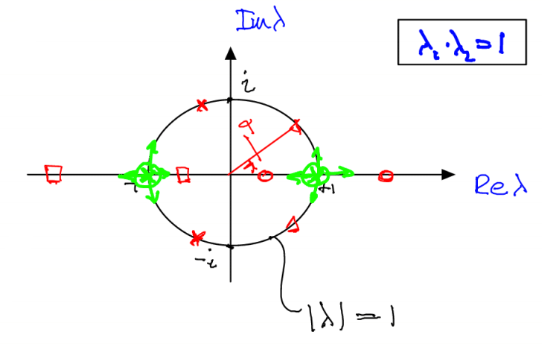
\includegraphics[width=0.4\textwidth]{figures/ch8/7poinc_eigv_config.png}
	\caption{All possible eigenvalue configurations of the linearized Poincaré map.}
	\label{fig:poinc_eigv_config}
\end{figure}

Next we examine what happens when we perturb homoclinic orbits. We recall the setting for homoclinic chaos in the Hamiltonian case with $H_1$ being $T$-periodic in $t$
\begin{align}
	\dot{x} = JD[H(x) + \varepsilon H_{1}(x,t)].
\end{align}
We assumed that the unperturbed system had a homoclinic obrbit and then asked if the unstable and stable manifolds of the perturbed system intersected then asked if the unstable and stable manifolds intersected using the Melnikov method, as sketched in Fig. \ref{fig:ham_melnikov_method}.
\begin{figure}[h!]
	\centering
	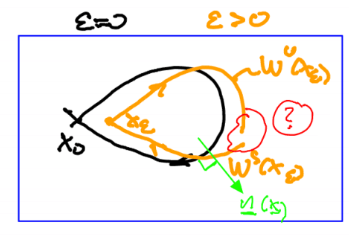
\includegraphics[width=0.4\textwidth]{figures/ch8/8ham_melnikov_method.png}
	\caption{The unperturbed $\varepsilon=0$ system with a homoclinic orbit in black and the perturbed $\varepsilon>0$ system in yellow, the Melnikov method analyzes if the unstable and stable manifold intersect.}
	\label{fig:ham_melnikov_method}
\end{figure}

\begin{proposition}[]
	The unstable manifold $W^{U}(x_{\varepsilon})$ and stable manifold $W^{S}(x_{\varepsilon})$ must intersect for $\varepsilon>0$.
\end{proposition}
\begin{proof}
	Assume contrarilty that for $\varepsilon>0$ the manifolds do not intersect. This leaves us with the image shown in Fig. \ref{fig:contradiction_assumption}.
	\begin{figure}[h!]
		\centering
		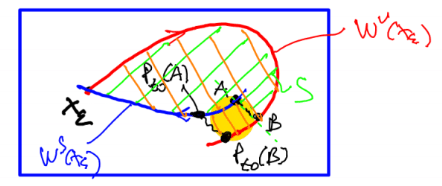
\includegraphics[width=0.4\textwidth]{figures/ch8/9contradiction_assumption.png}
		\caption{The image which we are left with if the two manifolds do not intersect.}
		\label{fig:contradiction_assumption}
	\end{figure}

	As in Fig. \ref{fig:contradiction_assumption}, denote by $A$ a poin in $ W^{S}(x_\varepsilon)$ and by $B$ a poin in $W^{U}(x_{\varepsilon})$. Then call the region $S$ the area enclosed by the curves of each manifold and the line $AB$. The region $S$ under the  Poincaré map now has a larger area than $S$, as can be seen by calculating:
\begin{align}
	\textrm{vol}[P_{t_0}(S) - S] =  \textrm{vol} [\overline{ABP_{t_0}(A)P_{t_0}(B)}] \neq 0.
\end{align}
This violates the area preservation property of the Poincaré map, and therefore leads to a contradiction.
\end{proof}

There are four possible types of intersection geometries: transverse (chaotic), topologically transverse (chaotic), tangency, and equality (no chaos). These are all illustrated in Fig. \ref{fig:intersection_types}. The tangency intersection lacks area preservation, and is also not possible.

\begin{figure}[h!]
	\centering
	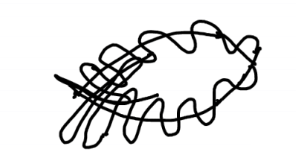
\includegraphics[width=0.45\textwidth]{figures/ch8/10intersection_geometry_A.png}
	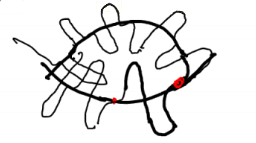
\includegraphics[width=0.4\textwidth]{figures/ch8/10intersection_geometry_B.png}
	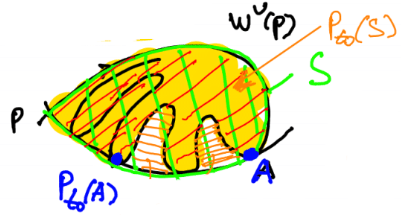
\includegraphics[width=0.45\textwidth]{figures/ch8/10intersection_geometry_C.png}
	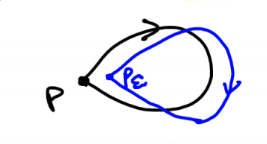
\includegraphics[width=0.4\textwidth]{figures/ch8/10intersection_geometry_D.png}
	\caption{The four types of intersection geometries, clockwise from the top-left: transverse, topologically transverse, tangent, and equal. The lack of area preservation for tangent intersection is visible by the existense of the intrusions which appear.}
	\label{fig:intersection_types}
\end{figure}

An equality intersection can occor when the Hamiltonian is conserved even after perturbation. This implies that all trajectories continue to remain confined to the level sets of $H$. 

As tangent intersections are not possible within the area preserving context, if $M(t_0) \neq 0$ then we must have homoclinic chaos. Thus in periodically forced Hamiltonian systems, chaos is generic!

\begin{proposition}[Recurrence]
	For an autonomous Hamiltonian system
	\begin{align}
		\dot{x}= JDH(x);\quad x \in \mathbb{R}^{2n},
	\end{align}
	if there exists a subset $S_0$ of $\mathbb{R}^{2n}$ which is compact, invariant, and has nonzero volume. Then for \underline{any} open set $U\subset S_0$ and \underline{any} time $T>0$, there exists an $x_0 \in U$ and $t>T$ such that $x(t;t_0, x_0)\in U$.	
\end{proposition}
This property is illustrated in Fig. \ref{fig:hamiltonian_recurrence}.
\begin{figure}[h!]
	\centering
	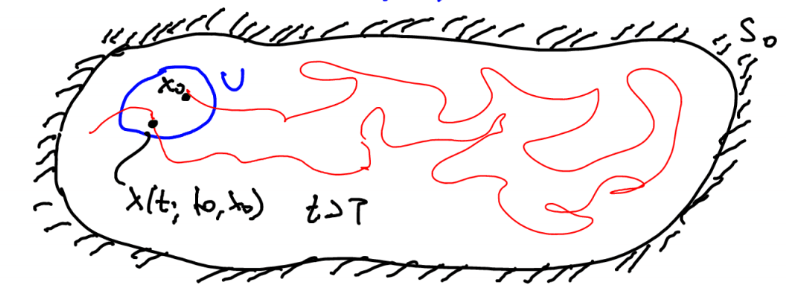
\includegraphics[width=0.7\textwidth]{figures/ch8/11hamiltonian_recurrence.png}
	\caption{A depiction of the recurrence property of autonoumous, area-preserving, Hamiltonian systems.}
	\label{fig:hamiltonian_recurrence}
\end{figure}
\begin{proof}
	The recurrence propery follows from the more general Poincaré Reccurence Theorem, which can be applied here as the flow map $F_{t_0}^{t}:x_0 \mapsto x(t;t_0, x_0)$ is volume preserving and invertible and $S_0$ is compact, invariant, and has nonzero volume.
\end{proof}
\begin{proposition}[Poincaré Recurrence theorem]
	For a compact domain $B$ with nonzero volume equipped with an invertible, volume preserving map $P:B\to B$, for any open subset $U\subset B$ there exists a $N \in \mathbb{N}^{+}$ such that
	\begin{align}
		\boxed{P^{N}(U) \cap U \neq \emptyset.}
	\end{align}
\end{proposition}
\begin{proof}
	Consider the sequence $U, P(U), P^{2}(U),\ldots$, we claim that at least two of these sets intersect. Towards a contradiction, assume that each set is disjoint, therefore we have
	\begin{align}
		\textrm{vol} [B] \geq  \textrm{vol} \left[ \bigcup_{i=0}^{\infty }P^{i}(U) \right] = \sum_{i=0}^{\infty }  \textrm{vol} \left[ P^{i}(U) \right] = \sum_{i=1}^{\infty } \ \textrm{vol} [U]= \infty .
	\end{align}
	The first inequality stems from the invariance of $B$, the second equality from the disjointness assumption, and the third from the volume preservation. This is clearly a contradiction as $B$ is compact and must have finite volume. Therefore there exist $m,n$ such that the intersection $P^{m}(U)\cap P^{n}(U)$ is non-empty. Call this intersection $A$ and assume without loss of generality that $n>m$. 

	For an $x \in A $ we know that $x\in P^{m}(U) $, thus $P^{-m}(x) \in U $, similarly we know $x\in P^{n}(u) $ so $P^{-m}(x)\in P^{n-m}(U) $. Putting these two facts together tells us that $P^{-m}(x) $ is an element of $U $ and $P^{n-m}(U)$, hence the intersection $U\cap P^{n-m}(U)$ cannot be empty. By calling $N=n-m$, we have shown the proposition.
\end{proof}
\begin{remark}[]
	There is a stronger version of Poincaré's Recurrence theorem, which states that almost all initial conditions return arbitrarily close to themselves. Here almost all is with respect to the assumed volume.
\end{remark}

\begin{ex}[Recurrence of the pendulum]
	For the pendulum, the area enclosed by an energy level set can be used as $S_0$. For large enough energy levels, this set may not be compact. This can be resolved by transforming the phase space $\mathbb{R}^{2}\to \mathcal{S}^{1}\times \mathbb{R}$ by taking advantage of the periodicity. This is shown in Fig. \ref{fig:pendulum_recurrence} where the importance of compactness and invariability are demonstrated as well.
	\begin{figure}[h!]
		\centering
		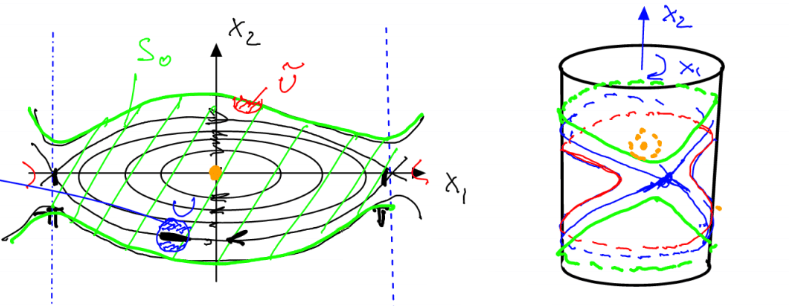
\includegraphics[width=0.75\textwidth]{figures/ch8/12pendulum_recurrence.png}
		\caption{The recurrence of the pendulum is depicited along with the phase space transformation. The recurrence in the standard phase space holds for all point in the set $U$ (blue), each element returns arbitrarily often. For the set $\tilde{U}$ (red), these points do not return infinitely often, and in fact never return in the base space. This is due to the fact that in the base space $S_0$ is not compact, if instead we identify the two dotted blue lines to transform the base space based on periodicity, we find that recurrence does hold.}
		\label{fig:pendulum_recurrence}
	\end{figure}
\end{ex}

\begin{ex}[Recurrence in non-smooth conservative systems]
	For a linear spring with a mass attached, which can bound off an elastic wall as the spring is expanded, we can also observe recurrence. Denoting the deviation of the mass by $q$ and the momentum by $m\dot{q}$ we still have recurrence under the map $P:x_0 \mapsto x(T;0, x_0)$, which is volume preserving. The dynamical system and phase space are illustrated in Fig. \ref{fig:bouncy_wall_spring}.
	 \begin{figure}[h!]
		\centering
		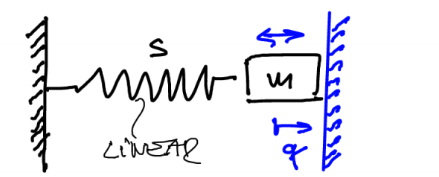
\includegraphics[width=0.45\textwidth]{figures/ch8/13bouncy_wall_spring_A.png}
		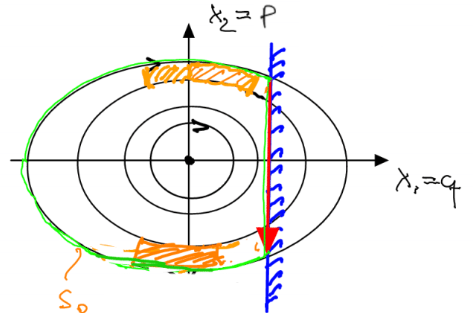
\includegraphics[width=0.4\textwidth]{figures/ch8/13bouncy_wall_spring_B.png}
		\caption{Left: A sketch of the dynamical system, with the elastic wall in blue. Right: The phase space of the dynamical system, with the red arrow designating that when the mass hits the wall (positive $x_2$) it immediately moves to the negative lower half (at the same absolute height) due to the elasticity. Furthermore, the volume preserving nature is shown by the two equal volume orange areas.}
		\label{fig:bouncy_wall_spring}
	\end{figure}
	
\end{ex}



